

%% This file was auto-generated by IPython.
%% Conversion from the original notebook file:
%%
\documentclass[11pt,english]{article}

%% This is the automatic preamble used by IPython.  Note that it does *not*
%% include a documentclass declaration, that is added at runtime to the overall
%% document.

\usepackage{amsmath}
\usepackage{amssymb}
\usepackage{graphicx}
\usepackage{grffile}
\usepackage{ucs}
\usepackage[utf8x]{inputenc}

% Scale down larger images
\usepackage[export]{adjustbox}

%fancy verbatim
\usepackage{fancyvrb}
% needed for markdown enumerations to work
\usepackage{enumerate}

% Slightly bigger margins than the latex defaults
\usepackage{geometry}
\geometry{verbose,tmargin=3cm,bmargin=3cm,lmargin=2.5cm,rmargin=2.5cm}

% Define a few colors for use in code, links and cell shading
\usepackage{color}
\definecolor{orange}{cmyk}{0,0.4,0.8,0.2}
\definecolor{darkorange}{rgb}{.71,0.21,0.01}
\definecolor{darkgreen}{rgb}{.12,.54,.11}
\definecolor{myteal}{rgb}{.26, .44, .56}
\definecolor{gray}{gray}{0.45}
\definecolor{lightgray}{gray}{.95}
\definecolor{mediumgray}{gray}{.8}
\definecolor{inputbackground}{rgb}{.95, .95, .85}
\definecolor{outputbackground}{rgb}{.95, .95, .95}
\definecolor{traceback}{rgb}{1, .95, .95}

% new ansi colors
\definecolor{brown}{rgb}{0.54,0.27,0.07}
\definecolor{purple}{rgb}{0.5,0.0,0.5}
\definecolor{darkgray}{gray}{0.25}
\definecolor{lightred}{rgb}{1.0,0.39,0.28}
\definecolor{lightgreen}{rgb}{0.48,0.99,0.0}
\definecolor{lightblue}{rgb}{0.53,0.81,0.92}
\definecolor{lightpurple}{rgb}{0.87,0.63,0.87}
\definecolor{lightcyan}{rgb}{0.5,1.0,0.83}

% Framed environments for code cells (inputs, outputs, errors, ...).  The
% various uses of \unskip (or not) at the end were fine-tuned by hand, so don't
% randomly change them unless you're sure of the effect it will have.
\usepackage{framed}

% remove extraneous vertical space in boxes
\setlength\fboxsep{0pt}

% codecell is the whole input+output set of blocks that a Code cell can
% generate.

% TODO: unfortunately, it seems that using a framed codecell environment breaks
% the ability of the frames inside of it to be broken across pages.  This
% causes at least the problem of having lots of empty space at the bottom of
% pages as new frames are moved to the next page, and if a single frame is too
% long to fit on a page, will completely stop latex from compiling the
% document.  So unless we figure out a solution to this, we'll have to instead
% leave the codecell env. as empty.  I'm keeping the original codecell
% definition here (a thin vertical bar) for reference, in case we find a
% solution to the page break issue.

%% \newenvironment{codecell}{%
%%     \def\FrameCommand{\color{mediumgray} \vrule width 1pt \hspace{5pt}}%
%%    \MakeFramed{\vspace{-0.5em}}}
%%  {\unskip\endMakeFramed}

% For now, make this a no-op...
\newenvironment{codecell}{}

 \newenvironment{codeinput}{%
   \def\FrameCommand{\colorbox{inputbackground}}%
   \MakeFramed{\advance\hsize-\width \FrameRestore}}
 {\unskip\endMakeFramed}

\newenvironment{codeoutput}{%
   \def\FrameCommand{\colorbox{outputbackground}}%
   \vspace{-1.4em}
   \MakeFramed{\advance\hsize-\width \FrameRestore}}
 {\unskip\medskip\endMakeFramed}

\newenvironment{traceback}{%
   \def\FrameCommand{\colorbox{traceback}}%
   \MakeFramed{\advance\hsize-\width \FrameRestore}}
 {\endMakeFramed}

% Use and configure listings package for nicely formatted code
\usepackage{listingsutf8}
\lstset{
  language=python,
  inputencoding=utf8x,
  extendedchars=\true,
  aboveskip=\smallskipamount,
  belowskip=\smallskipamount,
  xleftmargin=2mm,
  breaklines=true,
  basicstyle=\small \ttfamily,
  showstringspaces=false,
  keywordstyle=\color{blue}\bfseries,
  commentstyle=\color{myteal},
  stringstyle=\color{darkgreen},
  identifierstyle=\color{darkorange},
  columns=fullflexible,  % tighter character kerning, like verb
}

% The hyperref package gives us a pdf with properly built
% internal navigation ('pdf bookmarks' for the table of contents,
% internal cross-reference links, web links for URLs, etc.)
\usepackage{hyperref}
\hypersetup{
  breaklinks=true,  % so long urls are correctly broken across lines
  colorlinks=true,
  urlcolor=blue,
  linkcolor=darkorange,
  citecolor=darkgreen,
  }

% hardcode size of all verbatim environments to be a bit smaller
\makeatletter 
\g@addto@macro\@verbatim\small\topsep=0.5em\partopsep=0pt
\makeatother 

% Prevent overflowing lines due to urls and other hard-to-break entities.
\sloppy




\begin{document}




\section{Mathematics for Robotics and Control WS2013/14 - Assignment 6:
Signals and Systems}


\begin{codecell}


\begin{codeinput}
\begin{lstlisting}
import IPython.core.display
import sys
if not "win" in sys.platform and not "linux" in sys.platform:
    %pylab
else:
    %pylab inline
\end{lstlisting}
\end{codeinput}
\begin{codeoutput}


\begin{Verbatim}[commandchars=\\\{\}]
Populating the interactive namespace from numpy and matplotlib
\end{Verbatim}

\end{codeoutput}

\end{codecell}

\begin{center}\rule{3in}{0.4pt}\end{center}


\textbf{Modules}:

\begin{itemize}
\item
  control
\item
  numpy
\item
  scipy.io.wavfile
\item
  scipy.signal
\end{itemize}
\textbf{Functions}:

control:

\begin{itemize}
\item
  feedback, parallel, series, tf
\end{itemize}
scipy.io.wavfile:

\begin{itemize}
\item
  read
\end{itemize}

\begin{center}\rule{3in}{0.4pt}\end{center}

\paragraph{Assignment 6.1 \textbf{L1}}


Go to
{[}https://www.cds.caltech.edu/\_{murray/wiki/Control\_Systems\_Library\_for\_Python{]}(https://www.cds.caltech.edu/}murray/wiki/Control\_Systems\_Library\_for\_Python)
and download the Control Systems Library for Python. Use Anaconda's
\textbf{pip} to install the library into your local Anaconda
environment. Familiarize yourself with pip
\href{http://www.pip-installer.org/en/latest/}{here}. Please note that a
version of pip is \emph{already installed} in your Anaconda environment.

\textbf{Familiarize yourself with the control packages. Use
control.parallel, control.series, control.feedback and control.tf to
model the system depicted below. Obtain a SINGLE transfer function that
is equivalent to the complete system, i.e.~REDUCE the block diagram to a
single transfer function.}

\emph{Assignment 6.1 took me} \emph{minutes.}

\begin{codecell}


\begin{codeinput}
\begin{lstlisting}
IPython.core.display.Image(r"images/bdiag0002.png", embed=True)
\end{lstlisting}
\end{codeinput}
\begin{codeoutput}



\begin{center}
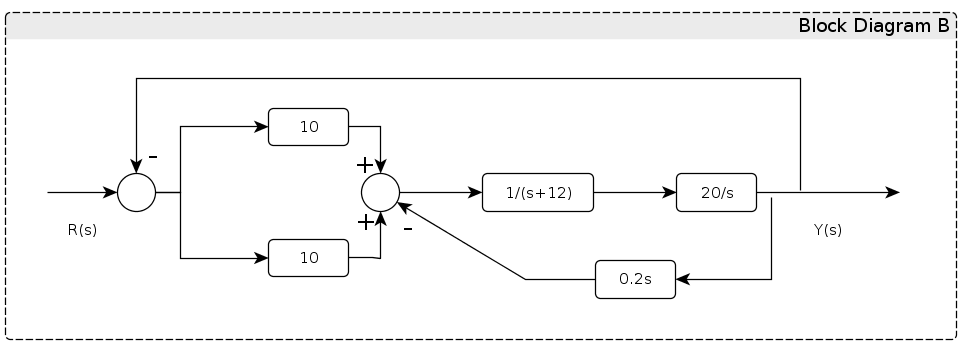
\includegraphics[max size={0.7\textwidth}{0.9\textheight}]{MRC_QUIGNONCHRISTOPHE_20140512_files/MRC_QUIGNONCHRISTOPHE_20140512_9_0.png}
\par
\end{center}


\end{codeoutput}

\end{codecell}

\begin{codecell}


\begin{codeinput}
\begin{lstlisting}
from control import *

ten = tf([10], [1])
par_left = parallel(ten, ten)
#print par_left

one_div_s_plus_twelve = tf([1], [1, 12])
twenty_s = tf([20], [1,0])
ser_right = series(one_div_s_plus_twelve, twenty_s)
#print ser_right

zero_point_two_s = tf([0.2, 0], [1])
#print zero_point_two_s

fb_right = feedback(ser_right, zero_point_two_s, -1)
#print fb_right

inner = series(par_left, fb_right)
#print inner

not_there = tf(1, 1)
complete = feedback(inner, not_there, -1)
print 'SOLUTION'
print complete
\end{lstlisting}
\end{codeinput}
\begin{codeoutput}


\begin{Verbatim}[commandchars=\\\{\}]
SOLUTION

       400
----------------
s^2 + 16 s + 400
\end{Verbatim}

\end{codeoutput}

\end{codecell}

\begin{center}\rule{3in}{0.4pt}\end{center}

\paragraph{Assignment 6.2 \textbf{L2}}


Find the Laplace transform Y(s) of the following functions:

\begin{enumerate}[1.]
\item
  $y(t) = e^{-2 \cdot t} \cdot u(t) + e^{-3 \cdot t} \cdot u(t)$
\item
  $y(t) = e^{-3 \cdot t} \cdot u(t) + e^{2 \cdot t} \cdot u(-t)$
\item
  $y(t) = e^{2 \cdot t} \cdot u(t) + e^{-3 \cdot t} \cdot u(-t)$
\end{enumerate}
Figure out how to obtain the Laplace transforms inside this notebook,
without doing it manually.

\begin{codecell}


\begin{codeinput}
\begin{lstlisting}
#can not be done[Ploeger, 2014]
#instead: study laplace transform
\end{lstlisting}
\end{codeinput}

\end{codecell}

\emph{Assignment 6.2 took me} \emph{minutes.}

\begin{center}\rule{3in}{0.4pt}\end{center}


Assignment 6.3 \textbf{L3}

Read \href{http://www.songho.ca/dsp/convolution/convolution.html}{this
article} about convolution, a very important concept in signal
processing. After you are done,
\href{http://www.dspguide.com/ch6/1.htm}{read some more}. Now, remember
that robot you were supposed to program to clean up after a party in one
of the earlier assignments? A few hours earlier, this robot was serving
as an electronic butler at said party and was supposed to answer the
phone when guests looking for directions were calling. The robot knows
the ringtone of it's owner's telephone quite well (file 00001.wav) and
is constantly listening to an audio stream of ambient sounds at the
party (file 00003.wav). Use convolution to determine the exact point in
time where the phone was ringing, relative to the beginning of the
ambient sounds. If your robot is especially clever, it might even take
on file 00002.wav, which corresponds to what the robot would hear at a
real party and is thus a little harder to process. This part of the
assignment is optional.

\begin{codecell}


\begin{codeinput}
\begin{lstlisting}
# Load Files
from scipy.io import wavfile as wf

ring_sample, ring = wf.read('00001.wav')
#stereo signal, drop one
ring = zip(*(ring))[0]
ring = list(ring)

#plot(zip(*(ring))[0])
#show()

party_sample, party = wf.read('00003.wav')
#stereo signal, drop one
party = zip(*(party))[0]
party = list(party)

party_sample2, party2 = wf.read('00002.wav')
#stereo signal, drop one
party2=zip(*(party2))[0]
\end{lstlisting}
\end{codeinput}

\end{codecell}

\begin{codecell}


\begin{codeinput}
\begin{lstlisting}
# Solution 6.3

#OPTIMIZATION
#could also be done live.

#absolute values
x = [abs(i) for i in party2] 
#Works even with on a good party!
h = [abs(i) for i in ring]

#mean of every n measurements
def downsample(l, n):
    chunks = [l[i:i+n] for i in range(0, len(l), n)]
    return map(median, chunks)

#Downsample the ratio is 44100/24000 which is 147/80
#This does not have to be exact
x = downsample(x, 80)
h = downsample(h, 147)

#Now the ringtone is ~140 measurements long
#we only look for one ring, so we have 3x3 times the chance to be right.
#xs = xs[6150:6290]#Ringtone in xs
h = h[70:210]#Ringtone in hs
#One ringtone block is aprox. 12 measuements wide
#so we can downsample once more
x = downsample(x, 12)
h = downsample(h, 12)

#Convolution
def convolute(x, h):
    #stretch h
    h = h + [0]*(len(x)-len(h))
    y=zeros_like(x)
    for n, _ in enumerate(x):
        for k in range(n):
            if n-k >= 0:
                y[n]=y[n] + x[k] * h[n-k]
        #MAGIC NUMBER HERE. I basically look for a drop.
        if n > 2 and y[n-1]/y[n]>1.2:
            #time relative to the soundsample
            p = float(n)/float(len(x))
            #Time depending on sample rate
            s = float(len(party2))/float(party_sample2)*p
            #We could also multiply the downsamplings
            print 'Ringtone after', s, 'seconds'
            break
    return y

#FUNCTION CALL
conv = convolute(x, h)

#OUTPUT
print 'X:'
plot(x)
show()

print 'H:'
plot(h)
show()

print 'CONVOLUTION:'
plot(conv)
show()

\end{lstlisting}
\end{codeinput}
\begin{codeoutput}


\begin{Verbatim}[commandchars=\\\{\}]
Ringtone after 28.76 seconds
X:
\end{Verbatim}

\begin{center}
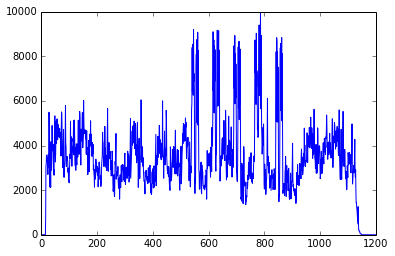
\includegraphics[max size={0.7\textwidth}{0.9\textheight}]{MRC_QUIGNONCHRISTOPHE_20140512_files/MRC_QUIGNONCHRISTOPHE_20140512_20_1.png}
\par
\end{center}

\begin{Verbatim}[commandchars=\\\{\}]
H:
\end{Verbatim}

\begin{center}
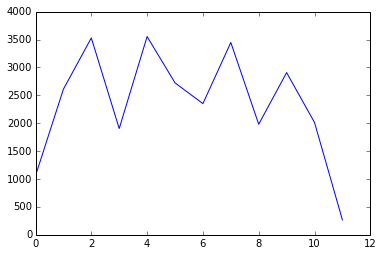
\includegraphics[max size={0.7\textwidth}{0.9\textheight}]{MRC_QUIGNONCHRISTOPHE_20140512_files/MRC_QUIGNONCHRISTOPHE_20140512_20_3.png}
\par
\end{center}

\begin{Verbatim}[commandchars=\\\{\}]
CONVOLUTION:
\end{Verbatim}

\begin{center}
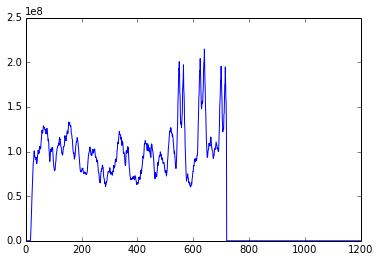
\includegraphics[max size={0.7\textwidth}{0.9\textheight}]{MRC_QUIGNONCHRISTOPHE_20140512_files/MRC_QUIGNONCHRISTOPHE_20140512_20_5.png}
\par
\end{center}

\end{codeoutput}

\end{codecell}

\emph{Assignment 6.3 took me} \emph{minutes.}

\begin{center}\rule{3in}{0.4pt}\end{center}


\emph{Use this button to create a .txt file containing the time in
minutes you spent working on the assignments. Make sure to include your
name in the textbox below. The file will be created in the current
directory.}

Student's name:



\end{document}

